\chapter{Implementace grafu}\label{Implementace grafu}
Hra Snake probíhá na čtvercovém hracím poli, kde se had pohybuje a snaží se sníst jablka, která se na něm objevují. Had se pohybuje postupně po jednotlivých políčkách, přičemž musí optimalizovat svou trasu tak, aby dosáhl jablka co nejefektivněji a zároveň se neuvěznil ve vlastní stopě. Abychom mohli efektivně řídit jeho pohyb a hledat nejkratší cesty, můžeme tento problém převést na graf. 

Hrací pole obsahuje \(n \times n\) políček, kde \(n\) je počet políček na jedné straně. Takové hrací pole dokážeme jednoduše reprezentovat jako čtvercový graf, což je graf, jehož vrcholy jsou uspořádány do pravidelné pravoúhlé mřížky o \(n^2\) vrcholech. Každý vrchol bude reprezen-\\tovat jedno políčko v hracím poli. Hrany grafu pak reprezentují možné pohyby hada mezi sousedními políčky. Každý vrchol má různý počet hran v závislosti na své poloze v mřížce. Do vrcholů reprezentující rohová políčka povedou dvě hrany. Uzly, které představují políčka na okraji hracího pole, budou napojeny třemi hranami a do vrcholů, které jsou uprostřed, vedou čtyři hrany. 

Tento graf lze reprezentovat dvěma způsoby: staticky, kdy se celý graf předem vygeneruje a uloží, nebo dynamicky, kdy se vrcholy a hrany vytvářejí pouze podle potřeby.

\section{Statická reprezentace}\label{Staticky}
V statické reprezentaci grafu si vygenerujeme najednou graf pro celé hrací pole a celý graf si uložíme do paměti. Tento graf nebudeme následně během hry nijak měnit. Pokud chceme provést změny v grafu, musíme celý graf smazat a vygenerovat nový graf, reflektují-\\ cí všechny požadované změny. 

Taková reprezentace je výhodná, pokud graf využíváme jako reprezentaci nějaké situace, která se nemění, tedy že se nemění graf, se kterým pracujeme. Např., když potřebujeme najít nejkratší cestu na mapách, stejnou mapu v tomto případě lze využít i opakovaně. Nejprve najdeme například nejkratší cestu domu a pokud budeme sledovat nalezenou trasu, cesta se v průběhu pohybu měnit nebude. Následně můžeme využít stejného grafu (mapy), abychom našli cestu z domova do školy, ze školy na kroužek atd. 

Výhodou takového přístupu tedy je, že generujeme pouze jeden graf. Nevýhodou je naopak potřeba generovat graf celý, tj. se všemi vrcholy a hranami. Když totiž hledáme nejkratší cestu (například pomocí algoritmu \(A*\)) z bodu $A$ do bodu $B$ v grafu, tak některé vrcholy pro nalezení nejkratší cesty nejen že nevyužijeme, ale ani je nebudeme kontrolovat. Při malém grafu to úplně nevadí, ale když je graf větší, může zabírat opravdu mnoho paměti. 

Uveďme si nyní, jak se dá statická reprezentace grafu použít v prostředí hry Snake při hledání nejkratší cesty od hlavy hada k jablku. 

\begin{figure}
    \centering
    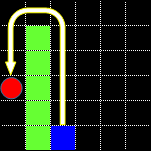
\includegraphics[width=0.5\linewidth]{Images/StaticGraphRepresentation.png}
    \caption{Nejkratší cesta od hlavy k jablku - statický graf, tělo hada - zelené čtverečky, hlava hada - modrý čtvereček, jablko - červené kolečko, šipka - nejkratší cesta od hlavy hada k jablku}
    \label{fig:StaticGraphRepresentation}
\end{figure}

Vygenerujeme si graf, kde budou propojeny všechny vrcholy tak, jak již bylo zmíněno v úvodu této kapitoly, s tím rozdílem, že do vrcholů grafu, ve kterých se nenachází tělo hada, nepovedou žádné hrany z okolních políček. Z těchto vrcholů povedou hrany pouze po směru pohybu hada do dalších částí jeho těla, tedy postupně propojíme orientovanými hranami jednotlivé části těla hada od ocasu až k hlavě. 

Tím docílíme toho, že algoritmus pro hledání nejkratší cesty se vyhne takovým cestám, ve kterých by had narazil sám do sebe. Algoritmus pro hledání nejkratší cesty tedy najde cestu podobnou jako na Obrázku~\ref{fig:StaticGraphRepresentation}. Vidíme, že nalezená cesta závisí pouze na počáteční situaci a algoritmus nebere vůbec v potaz, že se had bude hýbat (tedy, že v průběhu se může uvolnit prostor pro ještě kratší cestu).

Po vytvoření grafu algoritmus pro hledání nejkratší cesty najde nejkratší cestu s ohledem na počáteční situaci. To zároveň znamená, že pokud tělo hada momentálně zakrývá přímou cestu k jablku, tak ve statickém grafu to bude vnímáno tak, že bude cesta k jablku zakrytá pořád.

Ve hře Snake se had ovšem hýbe. Proto, pokud bude sledovat cestu nalezenou ve statickém grafu, bude ke konci obcházet překážku, která již reálně neexistuje. Při takovém přístupu budeme muset navíc po každém sebraném jablku vygenerovat nový graf, protože had neustále mění svoji pozici. Jak již bylo zmíněno, generování nového grafu je náročná operace a zejména při velkém grafu by trvala velmi dlouho. Proto statická reprezentace grafu pro simulaci hry Snake není úplně vhodná.

\section{Dynamická reprezentace}

V dynamické reprezentaci není nutné předem generovat celý graf, ale vrcholy se vytvářejí a prozkoumávají postupně během hledání nejkratší cesty. Každý vrchol obsahuje informace o svém předchozím stavu, tedy odkud jsme se do něj dostali, což umožňuje zpětně rekonstru-\\ ovat nalezenou cestu.

Tento proces probíhá iterativně – na začátku máme pouze výchozí stav (pozici hlavy hada) a postupně rozšiřujeme stavový prostor přidáváním sousedních vrcholů (možných pohybů hada). Každý nový stav odpovídá novému uspořádání herního pole po provedení daného tahu. Pokud narazíme na cílový stav (pozici jablka), můžeme zpětným sledováním předchozích stavů rekonstruovat nejkratší cestu.

Dynamická reprezentace tímto způsobem odpovídá principu prohledávání do šířky (BFS), kde se nejprve prozkoumávají všechny vrcholy v aktuální úrovni a teprve poté se přechází na další. BFS zajišťuje, že první nalezená cesta k cíli je zároveň nejkratší (pokud všechny tahy mají stejnou cenu), což je výhodné právě pro plánování pohybu hada. Hlavní rozdíl oproti statické reprezentaci je v tom, že zde nevytváříme celý graf dopředu, ale rozšiřujeme ho postupně podle potřeby. Tím se výrazně šetří paměť a umožňuje efektivní vyhledávání i ve větších prostředích. 
Podrobněji si to vysvětlíme na stejném příkladu jako při generování statického grafu (\ref{Staticky}).

\begin{figure}[h]
    \centering
    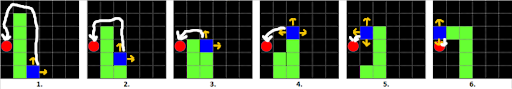
\includegraphics[width=\linewidth]{Images/DynamicGraphRepresentation.png}
    \caption{Nejkratší cesta od hlavy k jablku - dynamický graf, tělo hada - zelené čtverečky, hlava hada - modrý čtvereček, jablko - červené kolečko, žluté šipky - části grafu, které se aktuálně prozkoumávají pro hledání cesty, bílé šipky - aktuální nejkratší cesta od hlavy hada k jablku}
    \label{fig:DynamicGraphRepresentation}
\end{figure}

Máme dané pouze vrcholy reprezentující tělo hada a vrchol jablka. V prvním kroku na Obrázku~\ref{fig:DynamicGraphRepresentation} vidíme, že se had v dalším kroku dokáže pohnout pouze před sebe (rovně) nebo nahoru (doleva). To jsou vrcholy, které budeme prozkoumávat dál a také vrcholy, které vygenerujeme. Vygenerujeme je ovšem již pro situaci, která nastane, až se had na dané políčko posune. To znamená, že například pro možnost, kdy se had pohne nahoru (doleva), se každá část jeho těla posune o jedno políčko dopředu, na předcházející místo navazující části těla.

Druhý krok z Obrázku~\ref{fig:DynamicGraphRepresentation} tedy popisuje pozici hada, v případě, že se rozhodl pohnout v prvním kroku nahoru (doleva). Vidíme, že z této pozice se had může posunout buď doprava nebo nahoru (rovně). Postup z prvního kroku opakujeme a generujeme tak další možné stavy, dokud nenajdeme jablko. V každém stavu vygenerujeme pouze tělo hada a uložíme si k tomu i předchozí stav (stav, ze kterého vznikl aktuální stav).

Jak je vidět na Obrázku~\ref{fig:DynamicGraphRepresentation}, tento způsob reprezentace grafu nám umožňuje při hledání nejkratší cesty počítat i s pohybem hada v čase a díky tomu najít optimálnější cestu. Také nemusíme pokaždé, když hledáme novou cestu, vytvářet znovu celý graf, ale stačí nám vygenerovat pouze dílčí stavy, což je mnohem výhodnější nejen, co se týče paměti, ale i samotné rychlosti generování.